% chap2.tex
% 2010/12/03, v1.20

  \alphafootnotes
% for single-contributor books
  \chapterauthor{Magn\'us M\'ar Magn\'usson\footnotemark\
    and David Tranah\footnotemark}
  \chapteraffil{International Glaciological Society}

% for multi-contributor books
  \author[M\,M Magn\'usson and D\,A Tranah]
    {Magn\'us M\'ar Magn\'usson\footnotemark\
    and David Tranah\footnotemark}
  \authoraffil{International Glaciological Society}

  \chapter{The \cambridge\ class file in detail}

  \footnotetext[1]{Formerly of the Icelandic
    Meteorological Office, Reykjav\'\i k.}
  \footnotetext[2]{Supported by NSF Grant 43645.}
  \arabicfootnotes

  \contributor{Magn\'us M\'ar Magn\'usson
    \affiliation{International Glaciological Society,
      Scott Polar Research Institute,
      Lensfield Road, Cambridge CB2 1ER}}

  \contributor{David Tranah
    \affiliation{Cambridge University Press,
      The Edinburgh Building, Shaftesbury Road,
      Cambridge CB2 8RU}}

  \begin{chapterquote}
    The following notes may help you achieve the best effects with
    the \cambridge\ class file. The source code for this chapter
    quotation may be found in Section~\ref{chapterquote}.
  \source{Ali Woollatt}
  \end{chapterquote}

\section{Frenchspacing}

The \verb"\frenchspacing" option has been selected by default. This ensures that no extra space is inserted after full points, and is normal practice. If there is a strong reason for reversing this, you can key \verb"\nonfrenchspacing" in the preamble.

\section{Adding a subtitle to the front page}

The standard \verb"\title" command has been extended to take an optional argument which is then used as a subtitle on the main title page. For example, this document uses following title command:
\begin{verbatim}
  \title[Subtitle, If You Have One]
    {\LaTeXeintitle\ Guide for Authors using~the~\cambridge~Design}
\end{verbatim}

\section{Adding a blank page to your document}

Blank pages should not be numbered. If you require one, use the command \verb"\cleardoublepage", which has been redefined to start the next page on a recto, and if necessary, insert a totally blank verso page first.

% This section does not apply to the PT2 design
%\section{Adding a spanning rule to part and~chapter~openings}

%If your editor has asked you to use the spanning rule option for your book, it is called in as follows:\\[0.5\baselineskip]
%\verb"  \documentclass[spanningrule]{"\texttt{\cambridge}\verb"}"

\section{Chapter numbering}
If your book starts with an unnumbered chapter (e.g. \verb"\chapter*{Introduction}", then make all the numbered elements (e.g. section heads) unnumbered, by using \verb"\section*{...}". Otherwise, sections will be numbered 0.1, 0.2, etc.

\section{Section numbering}

\LaTeX\ provides five levels of section heads, and they are all defined in the \cambridge\ class file: \verb"\section", \verb"\subsection", \verb"\subsubsection", \verb"\paragraph", and \verb"\subparagraph". Numbers are given for the first three headings.

You can reduce the level of numbered section heads (it is not advisable to increase them). For instance, if you only want headings numbered down to subsections, add the following line to the preamble: \verb"\setcounter{secnumdepth}{2}". To number down to sections, make this \verb"\setcounter{secnumdepth}{1}", etc.

In addition to the standard section heads, \cambridge\ provides two further heads: \verb"\xhead" (used for examples, theorems, etc.) and \verb"\yhead" (used for solutions).


\section{Specifying running heads and toc entries}

\subsection{Single-contributor books}
\label{singlecontributor}

In \cambridge, chapter titles and section heads are used as running heads at the top of every page:
\begin{itemize}
\item chapter titles appear on even-numbered pages (versos), and
\item section heads appear on odd-numbered pages (rectos).
\end{itemize}
A problem with the standard version of \LaTeX\ has always been that the shortened versions of chapter and section titles, specified for running heads, have also been the entries for the toc. There are packages such as the memoir class which enable you to specify different toc entries, running head entries, and chapter titles. However, there is a simple way to add the verbose version of the chapter or section heads into the toc:
\begin{verbatim}
  \chapter[Toc entry]{Verbose chapter title}
  \chaptermark{Running head entry}

  \section[Toc entry]{Verbose section title
    \sectionmark{Running head entry}}
    \sectionmark{Running head entry}
\end{verbatim}
Note that for sections, you need the optional argument to \verb"\section", even if `Toc entry' is in fact the same text as `Verbose section title'. Also, the \verb"\sectionmark" has to be entered twice as shown, because the first \verb"\sectionmark" deals with the header of the page that the \verb"\section" command falls on, and the second deals with subsequent pages.

\subsection{Multi-contributor books}
\label{multicontributor}

Using the \cambridge\ multi-contributor option, author(s) name(s) and chapter titles are used as running heads at the top of every page:
\begin{itemize}
\item author(s) name(s) appear on even-numbered pages (versos), and
\item chapter titles appear on odd-numbered pages (rectos).
\end{itemize}
The author(s) names(s) may run to several lines, and contain new line commands (e.g. \verb"\\"), but the running head must be a single line. To enable you to specify the short form of the author(s) name(s) -- compulsory for the multi-contributor option -- the standard \verb"\author" command has been extended to take an optional argument to be used as the running head:
\begin{verbatim}
  \author[Author(s) name(s)]{The full author(s) name(s)}
\end{verbatim}
The following shows some coding for a chapter written by two authors, each of whom have footnotes. In this example, the authors' names will immediately follow the chapter title, and will read Magn\'us M\'ar Magn\'usson$^{a}$ and David Tranah$^{b}$. Their respective footnotes will be `$^{a}\enskip$Formerly of the Icelandic Meteorological Office, Reykjav\'\i k.' and `$^{b}\enskip$Supported by NSF~Grant 43645.' It is crucial that \verb"\author" precedes \verb"\chapter". If the authors have footnotes, you must start the chapter with \verb"\alphafootnotes", fill in the details for author(s), chapter title and author footnotes, then key \verb"\arabicfootnotes" to revert to arabic footnotes:
\begin{verbatim}
  \alphafootnotes
  \author[M\,M Magn\'usson and D\,A Tranah]
    {Magn\'us M\'ar Magn\'usson\footnotemark\
    and David Tranah\footnotemark}

  \chapter[Running head entry]
    {The \cambridge\ class file in detail}

  \footnotetext[1]{Formerly of the Icelandic
    Meteorological Office, Reykjav\'\i k.}
  \footnotetext[2]{Supported by NSF Grant 43645.}
  \arabicfootnotes
\end{verbatim}
Note that for multi-contributor books, the long version of the chapter title will always appear in the table of contents.

\section{Adding author(s) name(s) and affiliation(s)}

\subsection{Single-contributor books}

Sometimes, chapters in single-contributor books are written by different people. If you wish the authors and affiliations to appear beneath the chapter opening, as demonstrated in this chapter, key your chapter head as follows:
\begin{verbatim}
  \alphafootnotes
% for single-contributor books
  \chapterauthor{Magn\'us M\'ar Magn\'usson\footnotemark\
    and David Tranah\footnotemark}
  \chapteraffil{International Glaciological Society}

  \chapter{The \cambridge\ class file in detail}

  \footnotetext[1]{Formerly of the Icelandic
    Meteorological Office, Reykjav\'\i k.}
  \footnotetext[2]{Supported by NSF Grant 43645.}
  \arabicfootnotes
\end{verbatim}
If you have footnotes associated with the authors, you will also need to insert \verb"\alphafootnotes" and \verb"\arabicfootnotes", as shown.

Ensure that \verb"\chapterauthor" and \verb"\chapteraffil" are keyed before \verb"\chapter".


\subsection{Multi-contributor books}

If you wish the authors and affiliations to appear beneath the chapter opening, key your chapter head as follows:
\begin{verbatim}
  \alphafootnotes
% for multi-contributor books
  \author[M\,M Magn\'usson and D\,A Tranah]
    {Magn\'us M\'ar Magn\'usson\footnotemark\
    and David Tranah\footnotemark}
  \authoraffil{International Glaciological Society}

  \chapter{The \cambridge\ class file in detail}

  \footnotetext[1]{Formerly of the Icelandic
    Meteorological Office, Reykjav\'\i k.}
  \footnotetext[2]{Supported by NSF Grant 43645.}
  \arabicfootnotes
\end{verbatim}
If you have footnotes associated with the authors, you will also need to insert \verb"\alphafootnotes" and \verb"\arabicfootnotes", as shown.

Ensure that \verb"\author" and \verb"\authoraffil" are keyed before \verb"\chapter".

\section{Changing the level of entries in the table of~contents}
\label{changingentries}
The \cambridge\ design will, by default, list parts, chapters and sections in the table of contents. However, to improve the usefulness of this guide, we have used the command:
\begin{verbatim}
  \setcounter{tocdepth}{2}
\end{verbatim}
to increase this by one level, so the table of contents in this document also shows subsections.

\section{List of contributors}
\label{contrib}
The code for generating an automatic list of contributors should be entered after the author and chapter titles, as follows:
\begin{verbatim}
  \contributor{Magn\'us M\'ar Magn\'usson
    \affiliation{International Glaciological Society,
      Scott Polar Research Institute,
      Lensfield Road, Cambridge CB2 1ER}}

  \contributor{David Tranah
    \affiliation{Cambridge University Press,
      The Edinburgh Building, Shaftesbury Road,
      Cambridge CB2 8RU}}
\end{verbatim}
You then simply need to add the \verb"\listofcontributors" command after the table of contents (or after the artwork lists, if included) in the preamble, as follows:
\begin{verbatim}
  \tableofcontents
  \listoffigures
  \listoftables
  \listofcontributors
\end{verbatim}

\subsection{Note to editors regarding the list of contributors}

The contributors will appear in the same order as they are called in, since the list is generated in the same way as the table of contents. This means that at the final stage, the file will require editing to make the entries alphabetic.

Once you have a complete list of contributors, comment out the line which is generating them, and replace it as shown below:
\begin{verbatim}
  \tableofcontents
  \listoffigures
  \listoftables
 %\listofcontributors
  \editedlistofcontributors
\end{verbatim}
Next, rename the file with the extension \verb".loc" to \verb"editedloc.tex" (in the case of this guide, you would rename \texttt{\cambridge guide.loc} to \verb"editedloc.tex"). Edit this file as required, then run the file through \LaTeX\ once more, and the edited version will appear.

\section{Adding a Part quotation}
\label{partquotation}
The following code will give you the part quotation shown on page~\pageref{partquote}. Part quotations should be one paragraph long and precede the \verb"\part" command as follows:
\begin{verbatim}
  \partquote{I have called this principle...}{Charles Darwin}
    \label{partquote}
  \part{Getting started}
\end{verbatim}
\verb"\partquote" must have two arguments, so if you do not have a source for the quotation, replace \verb"{Charles Darwin}" with an empty set of braces~\verb"{}".

\section{Adding a Chapter quotation}
\label{chapterquote}
The following code will give you the chapter quotation and source shown at the beginning of this chapter. Chapter quotations should be one paragraph long:
\begin{verbatim}
  \begin{chapterquote}
    The following notes may help you achieve the best effects...
  \source{Ali Woollatt}
  \end{chapterquote}
\end{verbatim}

\section{Adding a `copyright' line to a chapter opening~page}
If you are publishing a single chapter, with permission from Cambridge University Press, you may be required to add a copyright line (and/or other information) to the footer of the chapter opening page. Add the following code somewhere on the first page of the chapter:
\begin{verbatim}
  \copyrightline{Reprinted from \textit{Mathematical
    Methods for Physics and Engineering} by Riley,
    Hobson and Bence \textcopyright~2010 Cambridge
    University Press.}
\end{verbatim}
Should the following chapter not require the copyright line, reverse this immediately before the next \verb"\chapter" command by using:
\begin{verbatim}
  \copyrightline{}
\end{verbatim}

\section{Lists}
\label{lists}

The \cambridge\ class provides the following standard list environments:
\begin{enumerate}
 \item numbered lists, created using the \verb"enumerate" environment;
 \item bulleted lists, created using the \verb"itemize" environment;
 \item labelled lists, created using the \verb"description" environment.
\end{enumerate}
The \verb"enumerate" environment numbers each list item with an arabic numeral followed by a full point; alternative styles can be achieved by inserting a redefinition of the number labelling command after the \verb"\begin{enumerate}". For example, a list numbered with lower-case letters inside parentheses can be produced. Because `(a)' is wider than a standard arabic digit, the label width has to be increased. This is achieved by specifying the widest label in the list inside square braces:
\begin{verbatim}
  \begin{enumerate}[(a)]
    \renewcommand{\theenumi}{(\alph{enumi})}
    \item estimate the fluctuations in the near-wall region\ldots
    \item subdue these near-wall fluctuations\ldots
  \end{enumerate}
\end{verbatim}
This produces the following list:
  \begin{enumerate}[(a)]
    \renewcommand{\theenumi}{(\alph{enumi})}
    \item estimate the fluctuations in the near-wall region\ldots
    \item subdue these near-wall fluctuations\ldots
  \end{enumerate}


\section{Extracts}
\label{extracts}

An extract may be included using the following coding:
\begin{verbatim}
  \begin{extract}
    In fact, neutron star matter is the most complex and
    fascinating state of matter that astronomers have yet
    discovered. The dense degenerate gas of neutrons appears
    to be superfluid, despite the very high temperatures~($10^6$\,K
    or higher) that we find inside neutron stars. (Bernard Schutz)
  \end{extract}
\end{verbatim}
The resulting extract is typeset in a slightly smaller font size, and indented:
  \begin{extract}
    In fact, neutron star matter is the most complex and
    fascinating state of matter that astronomers have yet
    discovered. The dense degenerate gas of neutrons appears
    to be superfluid, despite the very high temperatures~($10^6$\,K
    or higher) that we find inside neutron stars. (Bernard Schutz)
  \end{extract}

\section{Endnotes}

In addition to footnotes,\footnote{The footnote counter will be reset on chapters.} the \cambridge\ class provides a similar facility for endnotes. Their appearance depends on which option you are using:
\begin{enumerate}
\item for single-contributor books, the endnotes will be produced in the form of an unnumbered chapter at the end of the book;
\item for multi-contributor books, they are an unnumbered section at the end of each chapter.
\end{enumerate}
Endnotes are inserted into the text in a similar way to footnotes, but using the \verb"\endnote" command; for example,
\begin{verbatim}
  When the Richardson number\endnote{Lewis Fry Richardson
  (1881--1953).\label{richardson}} increases\ldots
\end{verbatim}
will produce `When the Richardson number\endnote{Lewis Fry Richardson (1881--1953).\label{richardson}} increases\ldots' in the text. Authors must choose between using footnotes and endnotes; do not use both.

\subsection{Single-contributor books}
Endnotes should be printed at the end of the book, after the appendices but before the bibliography and/or references.
\begin{verbatim}
    :
  \theendnotes
  \begin{thebibliography}{99}
    :
\end{verbatim}
The \verb"\theendnotes" command generates an unnumbered chapter which appears in the table of contents (see page~\pageref{richardson} for style).

\subsection{Multi-contributor books}

Endnotes should be printed at the end of the chapter using the same \verb"\theendnotes" command.


\section{Examples}
\label{examples}
Examples have rules both above and below. The default word `Example' may be replaced by `Alternative' by removing the comment symbol, as shown in the following list:
\begin{verbatim}
  \begin{examplelist}%[Alternative]
    \item Show that the geometrical definition of grad leads to the
          usual expression for $\nabla\phi$ in Cartesian coordinates.
    \solution{Solution}
          Consider a small rectangular volume element $\Delta V =
          \Delta x\,\Delta y\,\Delta z$ with its faces parallel to the
          $x,y,z$ coordinate surfaces and with the point $P$ at one
          corner. We must calculate\ldots

    \item Find the Fourier series of $f(x) =  x^3$ for $0 < x \leq 2$.
    \label{fourier}
    \solution{Solution}
          In the example discussed in the previous section we found
          the Fourier series for $f(x) = x^2$ in the required range.
          So, if we \textit{integrate} this term by term\ldots
  \end{examplelist}
\end{verbatim}
This will produce:
  \begin{examplelist}%[Alternative]
    \item Show that the geometrical definition of grad leads to the
          usual expression for $\nabla\phi$ in Cartesian coordinates.
    \solution{Solution}
          Consider a small rectangular volume element $\Delta V =
          \Delta x\,\Delta y\,\Delta z$ with its faces parallel to the
          $x,y,z$ coordinate surfaces and with the point $P$ at one
          corner. We must calculate\ldots

    \item Find the Fourier series of $f(x) =  x^3$ for $0 < x \leq 2$.
    \label{fourier}
    \solution{Solution}
          In the example discussed in the previous section we found
          the Fourier series for $f(x) = x^2$ in the required range.
          So, if we \textit{integrate} this term by term\ldots
  \end{examplelist}


\section{Exercises}

\subsection{Exercises at the end of sections}
\label{exendofsections}

Authors may use the \verb"exerciselist" environment which will typeset exercises at the end of each section. There is an option to add some useful text, such as `Exercise'; this is shown in the following example:
\begin{verbatim}
  \begin{exerciselist}[Exercise]
    \item Show that the link between shock formation and
          film rupture is invoked here because of the\ldots
    \item Show that the physical interpretation of\ldots
          \label{physi}
  \end{exerciselist}
\end{verbatim}
which will produce:
  \begin{exerciselist}[Exercise]
    \item Show that the link between shock formation and
          film rupture is invoked here because of the\ldots
    \item Show that the physical interpretation of\ldots
          \label{physi}
  \end{exerciselist}
As with all numbered environments, individual exercises (e.g. Exercise~\ref{physi}) can be cross-referenced.

\subsection{Exercises at the end of chapters}

If you would prefer to have the exercises at the end of each chapter, use the \verb"exercises" environment. This generates an entry in the table of contents and starts a new unnumbered section. For example,
\begin{verbatim}
  \begin{exercises}
    \item Let the film thickness be $h_0$,
          \begin{equation}
            h=h_0 H{\xi}.
          \label{exerciseeq}
          \end{equation}
          Integrating once\ldots
    \item Assuming the flow far away from\ldots
  \end{exercises}
\end{verbatim}
will produce:
  \begin{exercises}
    \item Let the film thickness be $h_0$,
          \begin{equation}
            h=h_0 H{\xi}.
          \label{exerciseeq}
          \end{equation}
          Integrating once\ldots
    \item Assuming the flow far away from\ldots
  \end{exercises}

\section{Problems}

\subsection{Problems at the end of sections}
\label{probendofsections}

Authors may use the \verb"problemlist" environment which will typeset problems at the end of each section. There is an option to add some useful text, such as `Problem'; this is shown in the following example:
\begin{verbatim}
  \begin{problemlist}[Problem]
    \item Show that in a theory with $\beta(g)=bg^2 + b'g^3 + b''g^4 +\cdots$,
          it is possible by a redefinition of the coupling constant
          to make the coefficient $b^n$ anything we want.
    \item Calculate the effective electric charge that should
          be used in studying processes at energy 100\,GeV, taking
          account of all known charged quarks and leptons with masses
          below 100\,GeV.
          \label{quarks}
  \end{problemlist}
\end{verbatim}
which will produce:
  \begin{problemlist}[Problem]
    \item Show that in a theory with $\beta(g)=bg^2 + b'g^3 + b''g^4 +\cdots$,
          it is possible by a redefinition of the coupling constant
          to make the coefficient $b^n$ anything we want.
    \item Calculate the effective electric charge that should
          be used in studying processes at energy 100\,GeV, taking
          account of all known charged quarks and leptons with masses
          below 100\,GeV.
          \label{quarks}
  \end{problemlist}
As with all numbered environments, individual problems (e.g. Problem~\ref{quarks}) can be cross-referenced.

\subsection{Problems at the end of chapters}

If you would prefer to have the problems at the end of each chapter, use the \verb"problems" environment. This generates an entry in the table of contents and starts a new unnumbered section. For example,
\begin{verbatim}
  \begin{problems}
    \item Show that if a functional $O$ satisfies the condition
          $(O,S)=i\Delta S$ and the action $S$ satisfies the
          quantum master equation then the quantum average
          $\langle O\rangle$ is independent of the gauge-fixing
          functional $\Psi$.
    \item Show that there is no simple Lie algrebra with just
          four generators.
  \end{problems}
\end{verbatim}
will produce:
  \begin{problems}
    \item Show that if a functional $O$ satisfies the condition
          $(O,S)=i\Delta S$ and the action $S$ satisfies the
          quantum master equation then the quantum average
          $\langle O\rangle$ is independent of the gauge-fixing
          functional $\Psi$.
    \item Show that there is no simple Lie algrebra with just
          four generators.
  \end{problems}


\section{Floating boxes}

The \cambridge\ design includes the use of boxes. These are floating objects, and are keyed in a similar way to tables. See Box~\ref{floatingbox} for an example (and note that you may have a `List of boxes' in the table of contents by adding \verb"\listoffloatingboxes" to the prelims.

  \begin{floatingbox}
    \processfloatingbox{A floating box --
      ensure that the title fits in one line}
    {The open string theory we have in our hands is the theory of
      strings on a D25-brane, a D-brane that fills all of the space
      dimensions. The D25-brane is a physical object, not just a
      mathematical construct, so it has a constant energy
      density~$T_{25}$ which, in fact, can be calculated exactly.
    \label{floatingbox}}
  \rule[-20pt]{\textwidth}{0.5pt}
\begin{verbatim}
  \begin{floatingbox}
    \processfloatingbox{A floating box --
      ensure that the title fits in one line}
    {The open string theory we have in our hands is the theory of
      strings on a D25-brane, a D-brane that fills all of the space
      dimensions. The D25-brane is a physical object, not just a
      mathematical construct, so it has a constant energy
      density~$T_{25}$ which, in fact, can be calculated exactly.
    \label{floatingbox}}
  \end{floatingbox}
\end{verbatim}
  \rule[20pt]{\textwidth}{0.5pt}
  \end{floatingbox}

\section{Figures}

The \cambridge\ class will cope with most positioning of your figures. As captions fall below figures, the figure must be included first, then the caption, then the label. This is illustrated in Figure~\ref{cantor}. The \verb"cantor1.eps" file has been called in by using \verb"\usepackage{rotating}" (which, in turn, calls in graphicx.sty) in the preamble.
  \begin{figure}
    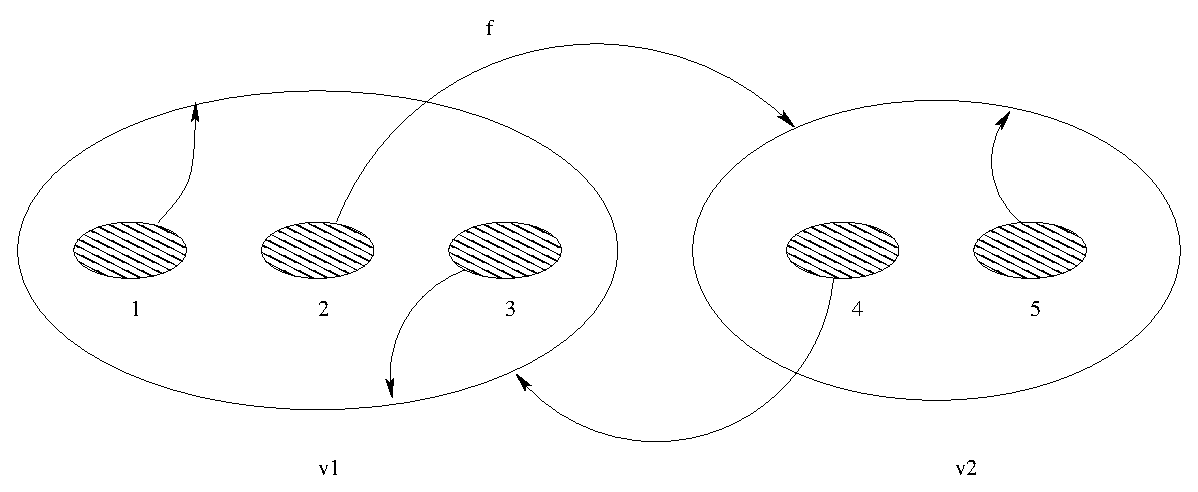
\includegraphics[scale=0.35]{cantor1.eps}
    \caption{A Cantor repeller. Figure captions will be
       flush-left and unjustified}
    \label{cantor}
\rule[-20pt]{\textwidth}{0.5pt}
\normalsize
\begin{verbatim}
  \begin{figure}
    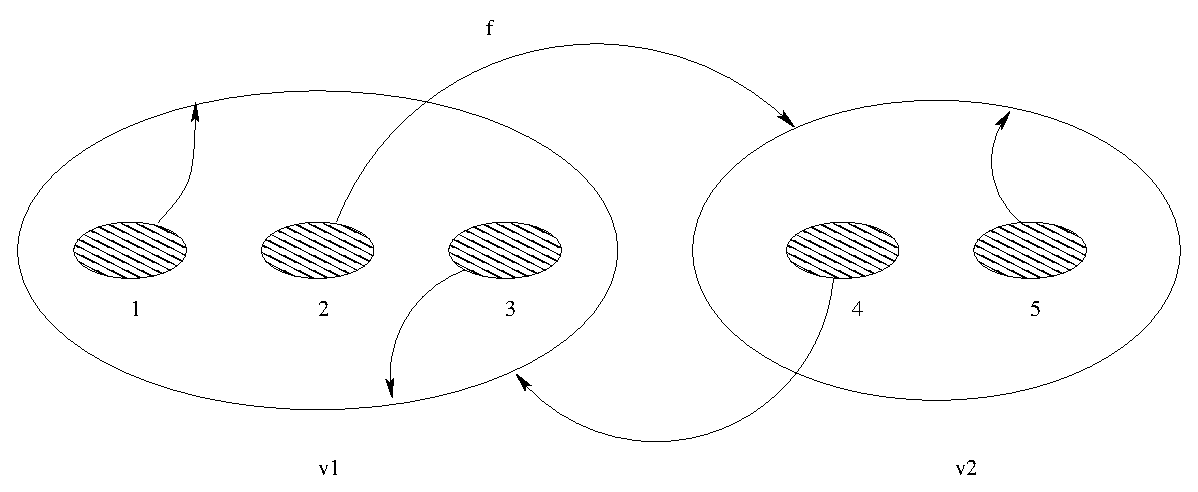
\includegraphics[scale=0.35]{cantor1.eps}
    \caption{A Cantor repeller. Figure captions will be
       flush-left and unjustified}
    \label{cantor}
  \end{figure}
\end{verbatim}
\rule[20pt]{\textwidth}{0.5pt}
  \end{figure}
Figures in the \cambridge\ design will all float to the top of the page; this has been necessary because of the coding required for very small figures (see Subsection~\ref{verysmallfigures}).

\subsection{Very small figures}
\label{verysmallfigures}

Figures less than 8.5pc (102pt) wide may be placed in the margin. \LaTeX\ has to treat them differently to achieve this, so you need to use \verb"\begin{verysmallfigure}..." \verb"\end{verysmallfigure}" \textit{and}
\begin{itemize}
\item place the figures in a vertical box of zero depth;
\item add \verb"\vfill".
\end{itemize}
If you don't do this, you will have vertical space appearing in the text beside the figure. A single figure would be typeset as follows:
\begin{verbatim}
  \begin{verysmallfigure}
  \vbox to0pt{%
    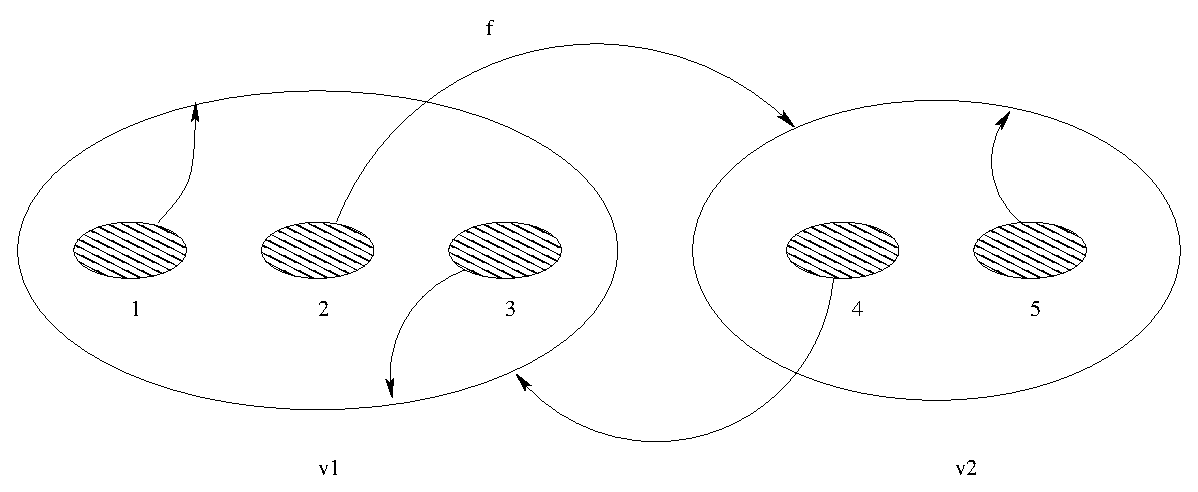
\includegraphics[width=8.5pc]{cantor1.eps}
    \caption{A typical margin figure}
    \label{typical}
  \vfill}
  \end{verysmallfigure}
\end{verbatim}
Note that since these figures take up zero vertical space, if you have two such figures on one page, you need to enclose both figures in one \verb"verysmallfigure" environment, and add vertical space between them. This is demonstrated in Figures~\ref{versionone} and~\ref{versiontwo}:
\begin{samepage}
\begin{verbatim}
  \begin{verysmallfigure}
  \vbox to0pt{%
    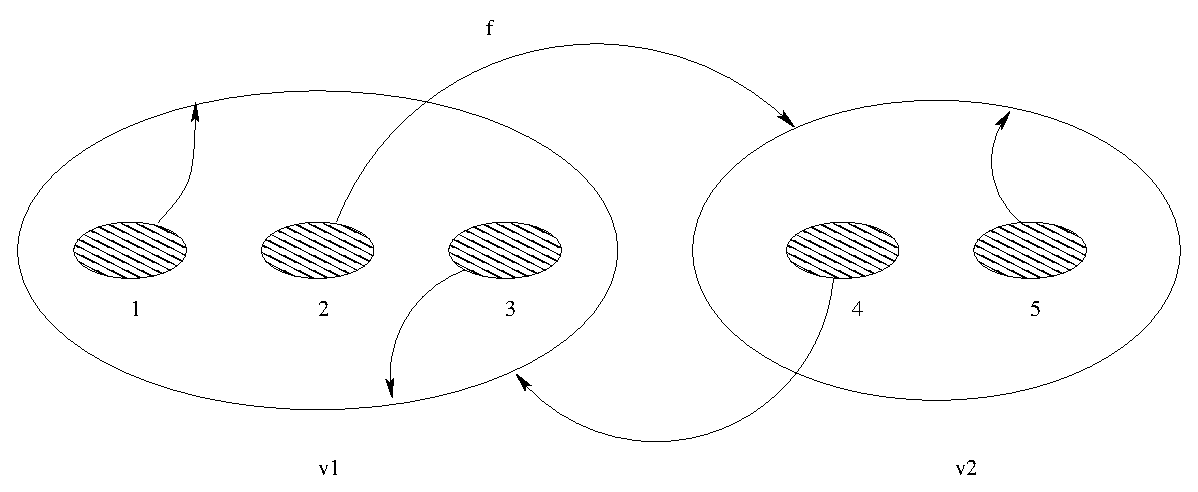
\includegraphics[width=8.5pc]{cantor1.eps}
    \caption{The first very small figure}
    \label{versionone}
      \vspace*{2\baselineskip}
    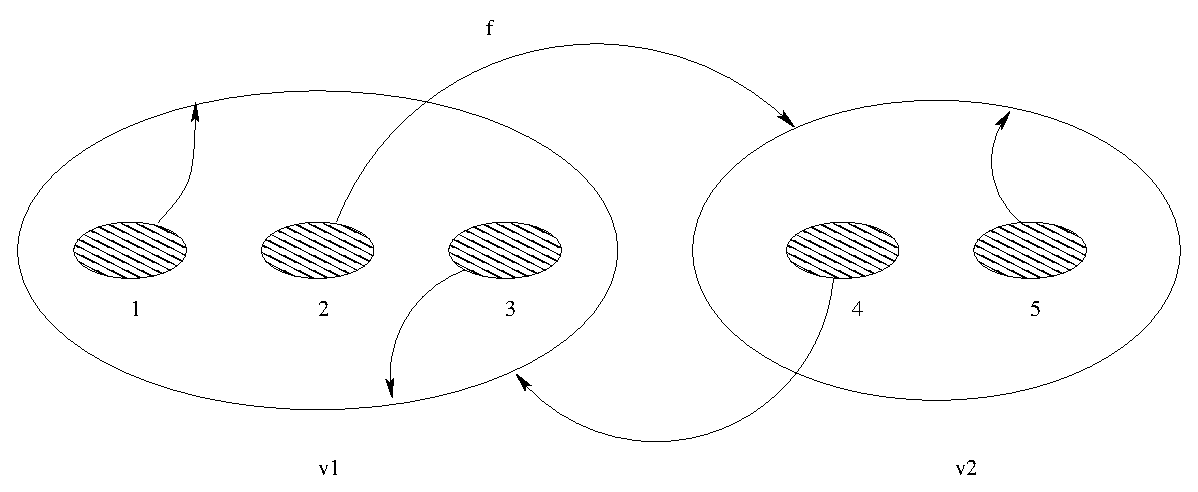
\includegraphics[width=8.5pc]{cantor1.eps}
    \caption{The second very small figure}
    \label{versiontwo}
  \vfill}
  \end{verysmallfigure}
\end{verbatim}
\end{samepage}
  \begin{verysmallfigure}
  \vbox to0pt{%
    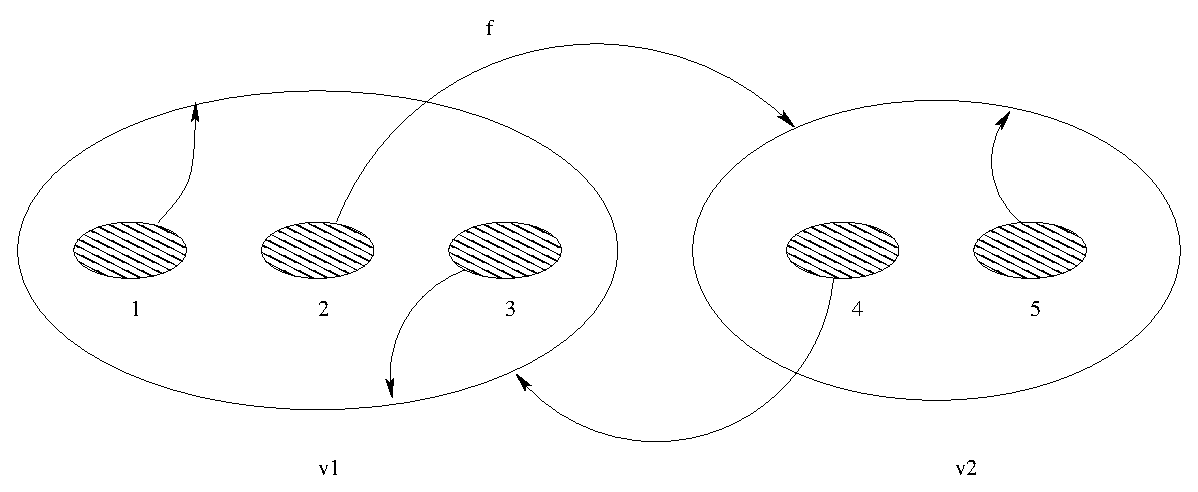
\includegraphics[width=8.5pc]{cantor1.eps}
    \caption{The first very small figure}
    \label{versionone}
      \vspace*{2\baselineskip}
    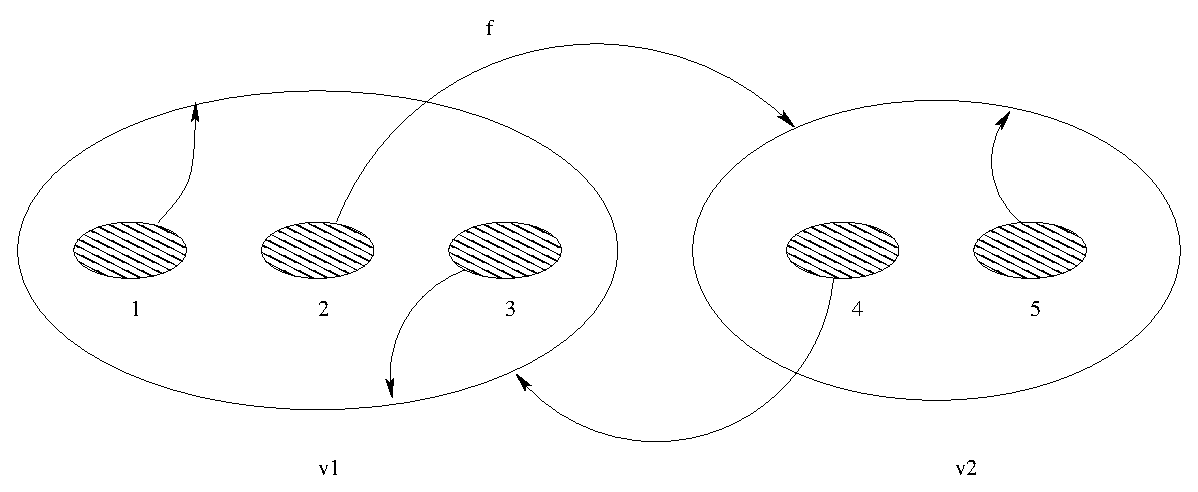
\includegraphics[width=8.5pc]{cantor1.eps}
    \caption{The second very small figure}
    \label{versiontwo}
  \vfill}
  \end{verysmallfigure}

\subsection{Wide figures 26--35pc}
\label{widefigures}

Figures may extend the full width of the page (35pc), as illustrated in Figure~\ref{anothercantor}. To achieve this, you must add \verb"\widefigure" before inserting the artwork (see the source code immediately below this figure).
  \begin{figure}% code for wide figures
    \widefigure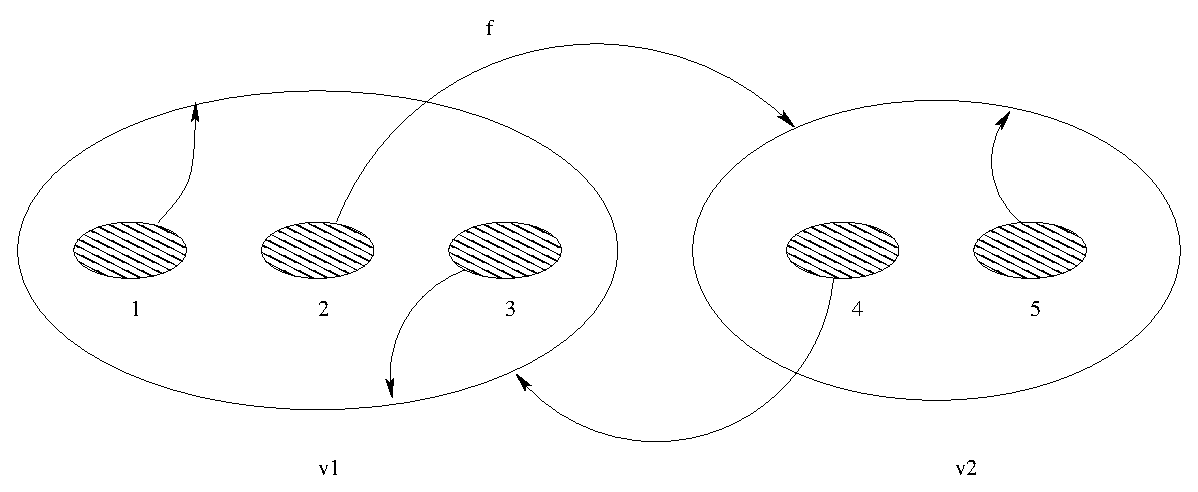
\includegraphics[width=35pc]{cantor1.eps}
    \caption{A wide figure}
    \label{anothercantor}
  \rule[-20pt]{\textwidth}{0.5pt}
\normalsize
\begin{verbatim}
  \begin{figure}% code for wide figures
    \widefigure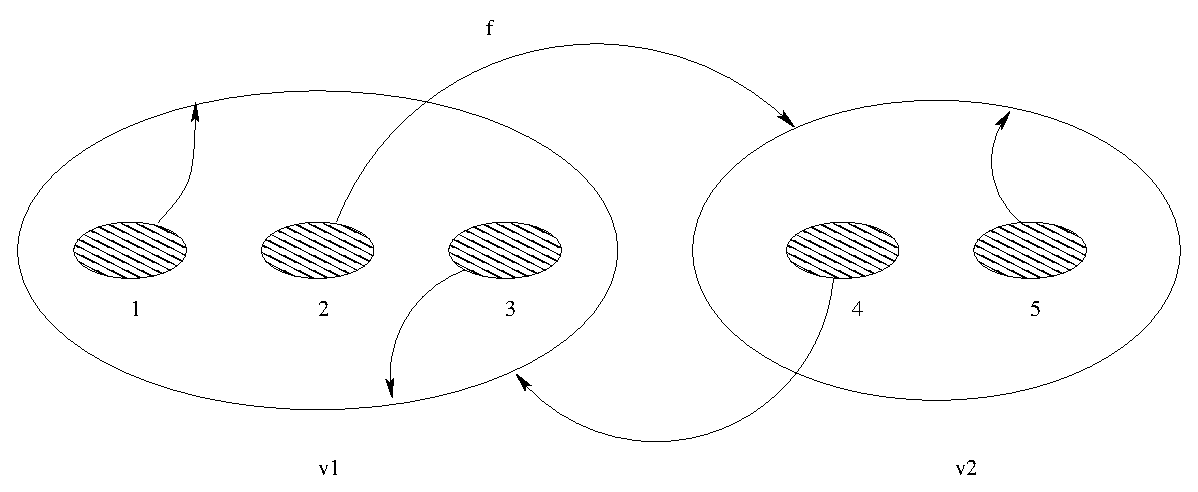
\includegraphics[width=35pc]{cantor1.eps}
    \caption{A wide figure}
    \label{anothercantor}
  \end{figure}
\end{verbatim}
  \rule[20pt]{\textwidth}{0.5pt}
  \end{figure}


\section{Tables}
\label{tables}

Due to the complex specification for tables in the \cambridge\ design, they need to be typeset slightly differently. Please refer to the source code immediately below Table~\ref{sample-table}, where you will find the following construction:
\begin{verbatim}
  \begin{table}
    \processtable
    {Table caption\label{transformation}}
    {\begin{tabular}...\end{tabular}}
  \end{table}
\end{verbatim}
In other words, they are typeset using \verb"\processtable" which contains 2~arguments.

The \cambridge\ class will cope with most positioning of your tables. Table captions must be included first, the the label, then the body of the table.

  \begin{table}
    \processtable
    {Note that table captions are typeset using~the
      \texttt{processtable} macro\label{sample-table}}
    {\addtolength\tabcolsep{2pt}% to stretch columns, if required
      \begin{tabular}{c@{\hspace{25pt}}ccc}
        Figure\footnote{\textit{Note:} All generalizations are false,
        including this one.} & $hA$ & $hB$ & $hC$\\
        \hline
        1 & $\exp\left(\pi i\frac58\right)$
          & $\exp\left(\pi i\frac18\right)$ & $0$\\[3pt]
        2 & $-1$    & $\exp\left(\pi i\frac34\right)$ & $1$\\[12pt]
        3 & $-4+3i$ & $-4+3i$ & $\frac74$\\[3pt]
        4 & $-2$    & $-2$    & $\frac54 i$\\
        \hline
      \end{tabular}}
  \rule[-20pt]{\textwidth}{0.5pt}
\begin{verbatim}
  \begin{table}
    \processtable
    {Note that table captions are typeset using~the
      \texttt{processtable} macro\label{sample-table}}
    {\addtolength\tabcolsep{2pt}% to stretch columns, if required
      \begin{tabular}{c@{\hspace{25pt}}ccc}
        Figure\footnote{\textit{Note:} All generalizations are false,
        including this one.} & $hA$ & $hB$ & $hC$\\
        \hline
        1 & $\exp\left(\pi i\frac58\right)$
          & $\exp\left(\pi i\frac18\right)$ & $0$\\[3pt]
        2 & $-1$    & $\exp\left(\pi i\frac34\right)$ & $1$\\[12pt]
        3 & $-4+3i$ & $-4+3i$ & $\frac74$\\[3pt]
        4 & $-2$    & $-2$    & $\frac54 i$\\
        \hline
      \end{tabular}}
  \end{table}
\end{verbatim}
  \rule[20pt]{\textwidth}{0.5pt}
  \end{table}
Tables in the \cambridge\ design will all float to the top of the page; this has been necessary because of the coding required for very small figures (see Section~\ref{verysmallfigures}).

\subsection{My vertical rules have disappeared}

Vertical rules in tables are not \cambridge\ style, and have been automatically removed; this gives your document a truly professional look. Instead of vertical rules, we recommend the use of extra horizontal space, see Section~\ref{addhoriz}. The rules have been removed by redefining the \verb"tabular" environment. The amended definition also inserts extra vertical space above and below the horizontal rules (produced by \verb"\hline").

If you really must have them reinstated, read Section~\ref{reinstate}.

\subsection{Reinstating the vertical rules}
\label{reinstate}
Authors can revert to the standard \LaTeX\ style, if necessary. Tables will take on a rather squashed appearance, as in the \LaTeX\ book, whereby there is no added space around horizontal rules. Add the command \verb"\reinstaterules" in the preamble, and re-run your files through \LaTeX.

\subsection{There is very little space around the rules in my~table}
Tables revert to the standard, rather squashed look of standard \LaTeX\ tables for two reasons:
\begin{enumerate}
  \item you are using \verb"array.sty"; or
  \item you have chosen to reinstate vertical rules (see Section~\ref{reinstate})
\end{enumerate}
In both cases, the tabular environment is redefined.


\subsection{Adding space between columns}
\label{addhoriz}
You can add space (2pt in this example) between every column using\linebreak \verb"\addtolength\tabcolsep{2pt}". However, if you only wanted to expand the space between columns~1 and~2 to~25pt, you would do this using\linebreak \verb"\begin{tabular}{@{}c@{\hspace{25pt}}ccc@{}}" (see Table~\ref{sample-table}).

\subsection{Adding space between rows}
If you need some form of separation between rows (for example, between rows~2 and~3 in the body of Table~\ref{sample-table}), adding \verb"[12pt]" immediately after the double backslash at the end of row~2 will add a 12pt vertical space (the equivalent of a blank line at this typesize). This is neater than adding another horizontal line.


\section{Landscape figures and tables, using rotating.sty}

Landscape figures and tables (floats) may be typeset using the \verb"rotating.sty" package. Note that the direction of rotation is always anti-clockwise, regardless of whether the rotated float lands on an even or odd page. To achieve this, be sure to add the optional argument \verb"[figuresright]" when calling in \verb"rotating.sty" (see below).

In addition to \verb"rotating.sty", you should also include \verb"floatpag.sty" and the command \verb"\rotfloatpagestyle{empty}". This combination ensures that headers and footers are removed from the float page:
\begin{verbatim}
  \usepackage[figuresright]{rotating}
  \usepackage{floatpag}
  \rotfloatpagestyle{empty}
\end{verbatim}
In some DVI previewers, floats may not appear rotated. If this happens, you need to convert the DVI file to PostScript or PDF.

Occasionally, when you convert a PostScript file to a PDF file, you may find that the page comes out upside-down. There will be a setting to change this. For instance, if you are using PDFCreator 0.9.7, choose the following options in this sequence:
\begin{description}
  \item Options -- Program -- PDF -- Auto-Rotate Pages: Change to `None'.
\end{description}
Other programs will have similar procedures.

\subsection{Coding for landscape figures}

The landscape figure (Figure~\ref{sidecantor}) was typeset using the following coding:
\begin{verbatim}
  \begin{sidewaysfigure}
    \centering
    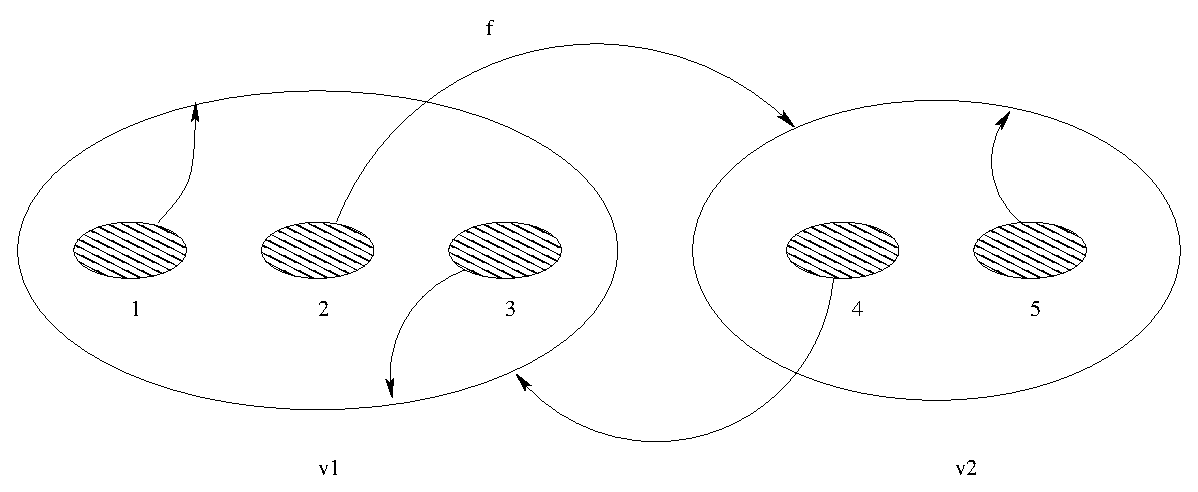
\includegraphics[scale=0.85]{cantor1.eps}
    \caption{A Cantor repeller: the landscape version}
    \label{sidecantor}
  \end{sidewaysfigure}
\end{verbatim}
  \begin{sidewaysfigure}
    \centering
    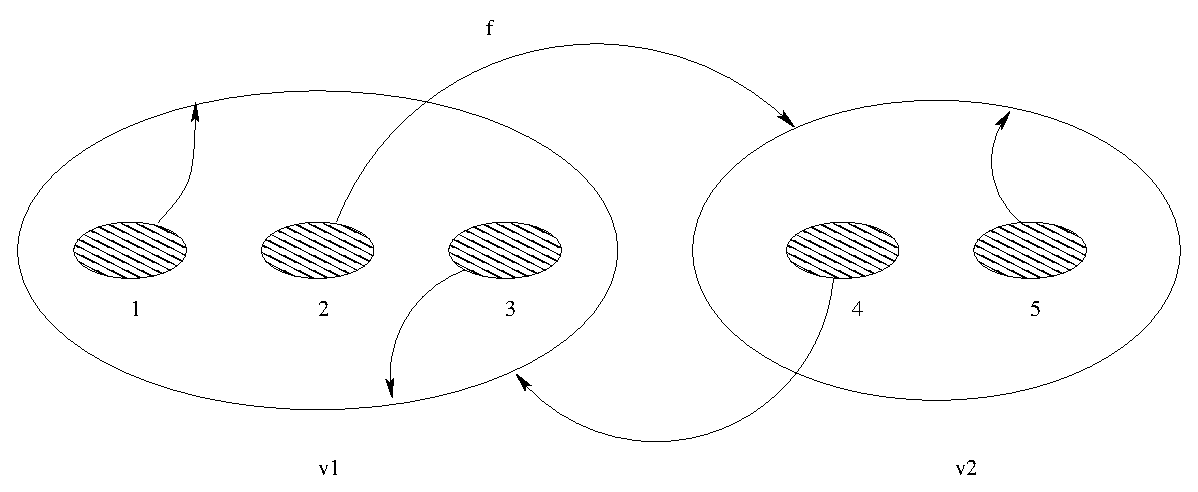
\includegraphics[scale=0.85]{cantor1.eps}
    \caption{A Cantor repeller: the landscape version}
    \label{sidecantor}
  \end{sidewaysfigure}

\subsection{Coding for landscape tables}

Table~\ref{sideways} has been produced using the following coding:
%
\begin{smallverbatim}
\begin{sidewaystable}
  \processtable
  {Grooved ware and beaker features, their finds and
    radiocarbon dates. For a breakdown of the pottery assemblages see
    Tables~I and~III; for the flints see Tables~II and~IV; for the animal
    bones see Table~V\label{sideways}}
  {\addtolength\tabcolsep{-2pt}
    \begin{tabular}{lcccllccccc}
    Context & Length & Breadth/  & Depth & Profile & Pottery & Flint & Animal
                                                     & Stone & Other & C14 Dates\\
    && Diameter &&&&& Bones\\[6pt]
    & m & m & m\\
    \hline\\[-5pt]
    \multicolumn{10}{l}{\textbf{Grooved Ware}}\\
    784 & --   & 0.9$\phantom{0}$ &0.18  & Sloping U & P1      & $\times$46
          & $\phantom{0}$$\times$8 && $\times$2 bone & 2150 $\pm$100\,\textsc{bc}\\
    785 & --   & 1.00             &0.12   & Sloping U & P2--4  & $\times$23
                                             & $\times$21 & Hammerstone & -- & --\\
    962 & --   & 1.37             &0.20   & Sloping U & P5--6  & $\times$48
                       & $\times$57 & --& --& 1990 $\pm$80\,\textsc{bc} (Layer 4)\\
    &&&&&&&&&& 1870 $\pm$90\,\textsc{bc} (Layer 1)\\
    983 & 0.83 & 0.73             &0.25   & Stepped U & --     & $\times$18
                                  & $\phantom{0}$$\times$8 & -- & Fired clay & --\\
    &&&&&&&&&&\\
    \multicolumn{10}{l}{\textbf{Beaker}}\\
    552 & --   & 0.68             & 0.12  & Saucer    & P7--14 & --           & --
                                                                     & -- &-- &--\\
    790 & --   & 0.60             & 0.25  & U         & P15    & $\times$12   & --
                                                        & Quartzite-lump & -- &--\\
    794 & 2.89 & 0.75             & 0.25  & Irreg.    & P16    & $\phantom{0}$$\times$3
                                                                & -- & -- &-- &--\\
    \end{tabular}}
\end{sidewaystable}
\end{smallverbatim}

\begin{sidewaystable}
  \processtable
  {Grooved ware and beaker features, their finds and
    radiocarbon dates. For a breakdown of the pottery assemblages see
    Tables~I and~III; for the flints see Tables~II and~IV; for the animal
    bones see Table~V\label{sideways}}
  {\addtolength\tabcolsep{-2pt}
    \begin{tabular}{lcccllccccc}
    Context & Length & Breadth/  & Depth & Profile & Pottery & Flint & Animal
                                                     & Stone & Other & C14 Dates\\
    && Diameter &&&&& Bones\\[6pt]
    & m & m & m\\
    \hline\\[-5pt]
    \multicolumn{10}{l}{\textbf{Grooved Ware}}\\
    784 & --   & 0.9$\phantom{0}$ &0.18  & Sloping U & P1      & $\times$46
          & $\phantom{0}$$\times$8 && $\times$2 bone & 2150 $\pm$100\,\textsc{bc}\\
    785 & --   & 1.00             &0.12   & Sloping U & P2--4  & $\times$23
                                             & $\times$21 & Hammerstone & -- & --\\
    962 & --   & 1.37             &0.20   & Sloping U & P5--6  & $\times$48
                       & $\times$57 & --& --& 1990 $\pm$80\,\textsc{bc} (Layer 4)\\
    &&&&&&&&&& 1870 $\pm$90\,\textsc{bc} (Layer 1)\\
    983 & 0.83 & 0.73             &0.25   & Stepped U & --     & $\times$18
                                  & $\phantom{0}$$\times$8 & -- & Fired clay & --\\
    &&&&&&&&&&\\
    \multicolumn{10}{l}{\textbf{Beaker}}\\
    552 & --   & 0.68             & 0.12  & Saucer    & P7--14 & --           & --
                                                                     & -- &-- &--\\
    790 & --   & 0.60             & 0.25  & U         & P15    & $\times$12   & --
                                                        & Quartzite-lump & -- &--\\
    794 & 2.89 & 0.75             & 0.25  & Irreg.    & P16    & $\phantom{0}$$\times$3
                                                                & -- & -- &-- &--\\
    \end{tabular}}
\end{sidewaystable}

  \begin{summary}
    A summary may be added at the end of each chapter using the
    coding below. The heading is a numbered section head; the text
    is slightly larger and sans-serif.
  \end{summary}
\begin{verbatim}
  \begin{summary}
    A summary may be added at the end of each chapter using the
    coding below. The heading is a numbered section head; the text
    is slightly larger and sans-serif.
  \end{summary}
\end{verbatim}
\endinput

